\chapter{Conception and Design}

\section{Introduction}
This chapter translates the theoretical spine-leaf architecture from Chapter 1 into a concrete design. We detail the topology, VLANs, IP addressing, VRRP, MLAG, security zones, and UML models. The resulting blueprint guides implementation in Chapter 3.
\section{Architecture Overview}

\subsection{Spine-Leaf Topology\hyperref[def:hld]{\underline{ (HLD)}}}
The architecture adopts a Spine-Leaf model across four virtual cabinets: A, B, C, and D. Each cabinet is equipped with two ToR switches acting as leaf nodes, giving a total of eight ToR switches at the access layer. The cabinets are interconnected through two EoR core switches acting as spine nodes, each connected to all eight ToR switches, ensuring that any server can reach any other server with minimal hops and maximum redundancy.
\subsection{Justification of Choice}
The Spine-Leaf model was chosen for this project because it reflects the architecture for modern enterprise data centers. It addresses the performance and scalability requirements of a multi-cabinet infrastructure while maintaining the security and zone separation necessary for hosting services across different trust levels, from internal database and application services to externally accessible web services in the DMZ. These choices transform a basic topology into a production-ready, carrier-grade data center blueprint.
% Landscape HLD page (rotated figure on its own page — do NOT use [H] with sidewaysfigure)
\clearpage
\thispagestyle{plain}
\begin{sidewaysfigure}[p]
    \centering
    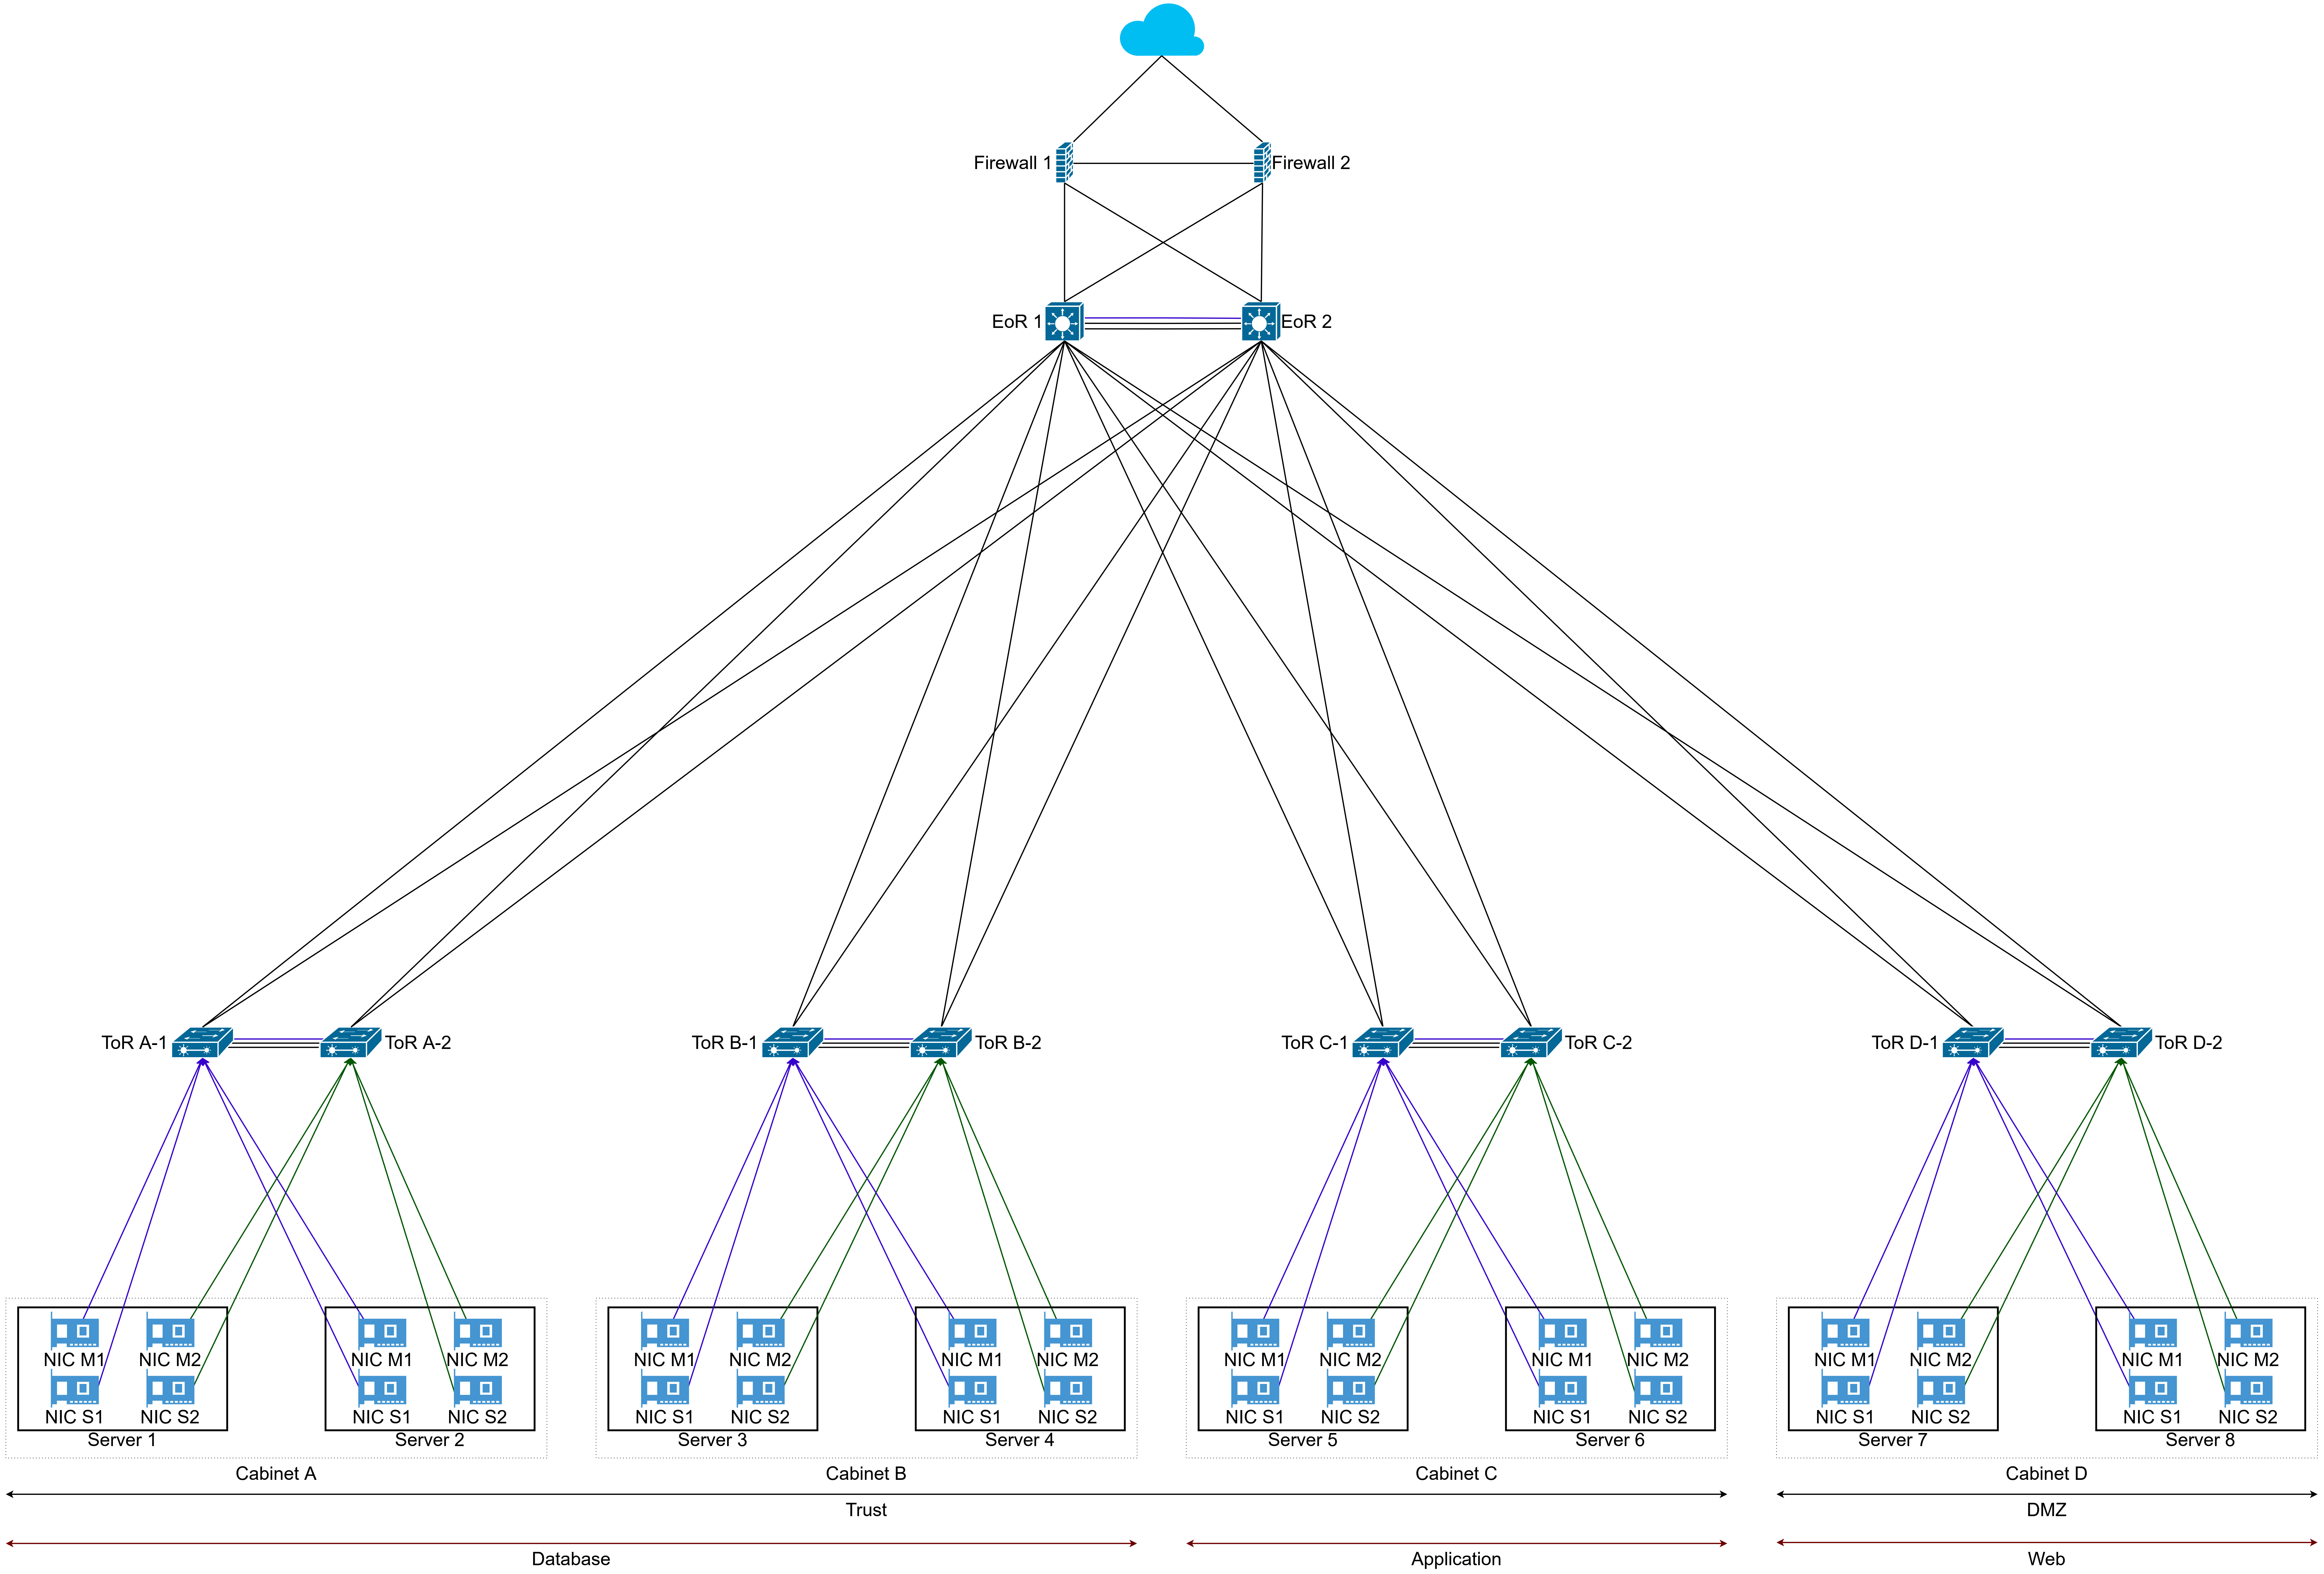
\includegraphics[width=0.92\textheight,keepaspectratio]{figures/HLDV4.drawio.png}
    \caption{Spine-Leaf topology of the proposed data center.}
    \label{fig:topology}
\end{sidewaysfigure}
\FloatBarrier
\clearpage

\subsection{Leaf Layer}
\begin{figure}[H]
    \centering
    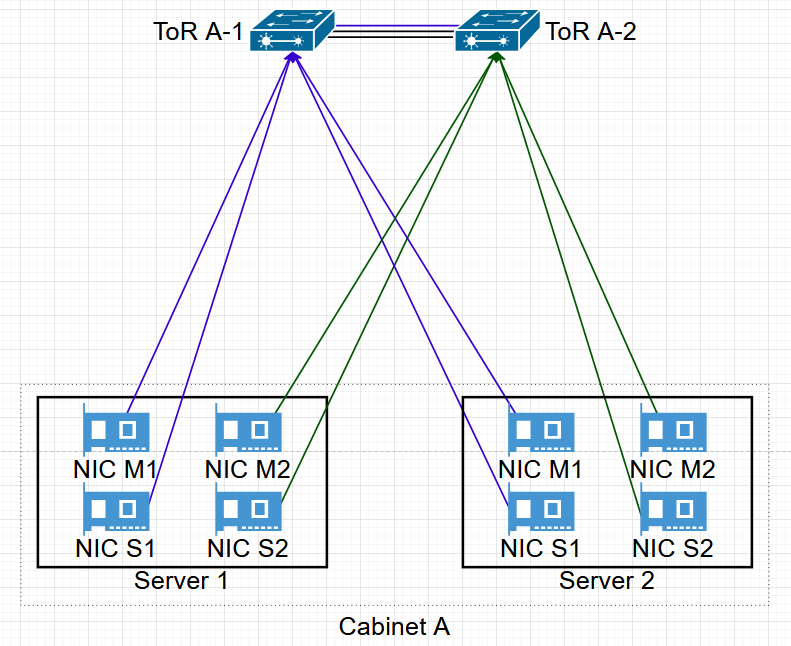
\includegraphics[width=0.45\textwidth,interpolate=false]{figures/leaf_layer.png}
    \caption{Leaf Layer}
    \label{fig:leaf-layer}
\end{figure}
\textbf{1. Cabinets and Servers:} The physical infrastructure consists of four server cabinets (A, B, C, and D). Each cabinet houses two servers, resulting in a total of eight physical servers. Cabinet A contains Servers 1 and 2; Cabinet B contains Servers 3 and 4; Cabinet C contains Servers 5 and 6; Cabinet D contains Servers 7 and 8.\\
Each server contains two active network cards (\hyperref[def:management]{\underline{M1}} and \hyperref[def:service]{\underline{S1}}) and two backup network cards (M2 and S2):\\
- M: Management network card, used by the system administrator to access the server for configuration.\\
- S: Service network card, used for application and production traffic between servers and services.\\
\textbf{2. ToR Switches:} Each cabinet is served by two ToR switches, one active and one standby, providing local connectivity for the servers within that cabinet. In each cabinet:\\
- ToR X-1 (active) connects to the two active network cards (M1 and S1) in the two servers in that cabinet.\\
- ToR X-2 (standby) connects to the two backup network cards (M2 and S2) in the two servers in that cabinet.\\
ToRs A-Y connect to the two servers in Cabinet A, ToRs B-Y connect to the two servers in Cabinet B, ToRs C-Y connect to the two servers in Cabinet C, ToRs D-Y connect to the two servers in Cabinet D.
\subsection{Spine Layer}
\begin{figure}[H]
    \centering
    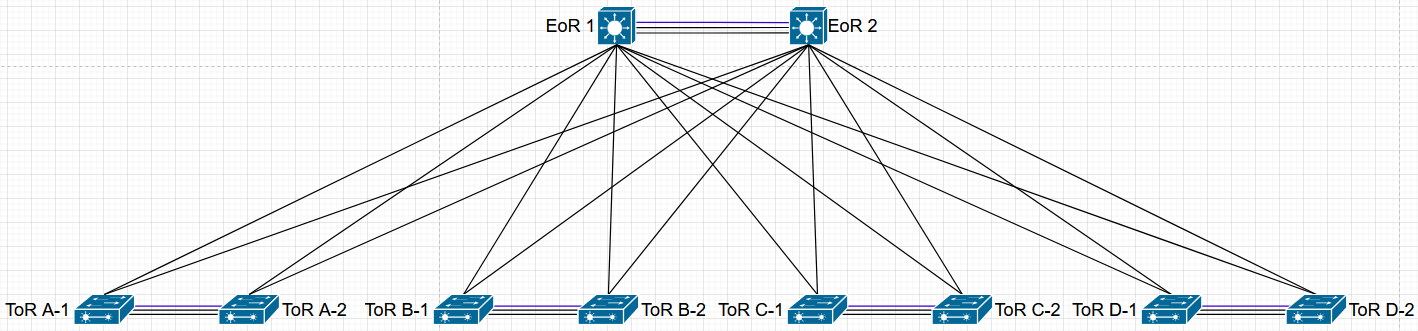
\includegraphics[width=0.75\textwidth,interpolate=false]{figures/spine_layer.png}
    \caption{Spine Layer}
    \label{fig:spine-layer}
\end{figure}
\textbf{EoR Switches}: All ToR switches uplink to the core layer, which consists of two End of Row (EoR) switches. These serve as the aggregation point for the entire server farm.\\
- EoR 1 and EoR 2 are configured in a high-availability (active/standby) pair.\\
- Each ToR maintains a connection to both EoR 1 and EoR 2. This ensures that if the active path fails, traffic can instantly switch to the standby core switch.\\
- A direct link exists between EoR 1 and EoR 2 to facilitate synchronization and failover detection (heartbeat).
\subsection{Network Edge}
\begin{figure}[H]
    \centering
    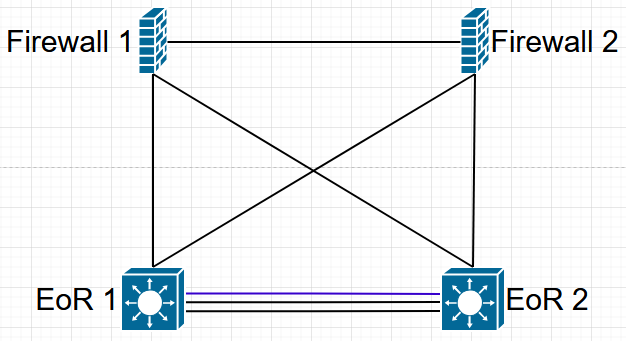
\includegraphics[width=0.45\textwidth,interpolate=false]{figures/network_edge.png}
    \caption{Network Edge}
    \label{fig:network-edge}
\end{figure}
\textbf{Firewalls:} The core switches connect directly to the network security layer, which is comprised of a pair of firewalls.\\
- Firewall 1 (Active) and Firewall 2 (Standby) provide north-south security for the server traffic.\\
- Both EoR 1 and EoR 2 are connected to both Firewall 1 and Firewall 2, eliminating a single point of failure in the uplink path.\\
- A direct link connects Firewall 1 and Firewall 2 to maintain session state synchronization and monitor health for seamless failover.\\
\subsection{Cloud Connection}
\begin{figure}[H]
    \centering
    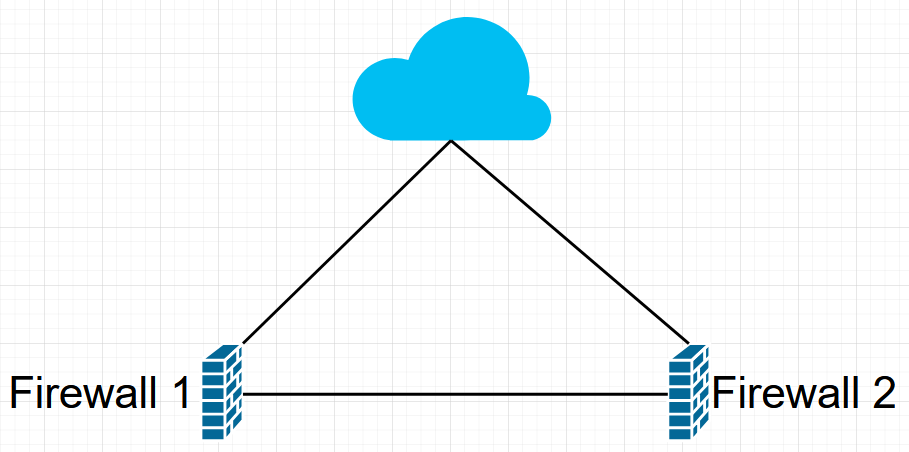
\includegraphics[width=0.45\textwidth,interpolate=false]{figures/cloud_connection.png}
    \caption{External cloud and network access}
    \label{fig:cloud-edge}
\end{figure}
The two perimeter firewalls connect the internal network to the external cloud network. All inbound and outbound traffic between the internal environment and the external network traverses these firewalls, where untrusted traffic is inspected and filtered according to security policies.\\
\subsection{Cabinet Structure}
The physical architecture is organized into four cabinets, each representing a specific function and security zone:

\begin{table}[htbp]
    \centering
    \caption{Cabinet organization by zone and function}
    \label{tab:cabinets}
    \begin{tabular}{|c|c|c|c|c|c|}
        \hline
        \textbf{Cabinet} & \textbf{Zone} & \textbf{Function} & \textbf{Servers} & \textbf{ToR Pair} & \textbf{VLANs} \\
        \hline
        A & Trust & Database & 2 servers & A-1, A-2 & 110, 120 \\
        B & Trust & Database & 2 servers & B-1, B-2 & 110, 120 \\
        C & Trust & Application & 2 servers & C-1, C-2 & 110, 130 \\
        D & DMZ & Web & 2 servers & D-1, D-2 & 210, 220 \\
        \hline
    \end{tabular}
\end{table}
Each cabinet contains two servers with four \hyperref[def:nic]{\underline{NICs}} per server and two ToR switches. The ToR switches are configured as an MLAG pair, operating in active-standby mode with one switch active and one standby.
 \section{Requirements Specification}
 \subsection{Actors:}
The system supports several categories of actors, each with rights and responsibilities adapted to their role. Six primary actors interact with the data center system, as summarized in Table~\ref{tab:actors}.

\begin{table}[htbp]
    \centering
    \caption{Primary actors of the data center system}
    \label{tab:actors}
    \begin{tabular}{|l|p{0.62\textwidth}|}
        \hline
        \textbf{Actor} & \textbf{Role and responsibilities} \\
        \hline
        External User & Client accessing web services hosted in the DMZ zone via HTTPS. \\
        \hline
        IT Administrator & Performs user authentication and monitors cabinet health across all four cabinets. \\
        \hline
        Network Admin & Configures switches, VLANs, VRRP redundancy, MLAG active-standby pairs, and trunk/access ports. \\
        \hline
        System Admin & Manages server virtual machines and multi-NIC configuration on Linux servers. \\
        \hline
        Security Admin & Manages firewall rules and enforces DMZ/Trust zone separation with default-deny policies. \\
        \hline
        Super Admin & Has full system access and inherits all capabilities from Network, System, Security, and IT Administrators. \\
        \hline
    \end{tabular}
\end{table}
\subsection{Functional Requirements}
The data center must fulfill the following functional requirements:\\
- The system must isolate web servers from application and database servers using firewall-enforced DMZ and Trust zones.\\
- The system must provide redundant gateway IPs so that server connectivity continues in case of failure.\\
- The system must support automatic failover between redundant ToRs, EoRs and firewalls with zero packet loss.\\
- The system must allow IT administrators to remotely configure all network devices via SSH on a dedicated management VLAN.\\
- The system should be ready for clients to deploy their own applications (web, application, and database) on the infrastructure.
\subsection{Non-Functional Requirements}
Non-functional requirements define the quality expectations and overall constraints of the data center. The main non-functional requirements identified are:\\
- \textbf{Redundancy:} No single point of failure at any layer. Spine, leaf, servers, and firewalls must all have redundancy.\\
- \textbf{Security:} DMZ and Trust zones must be strictly separated by firewall policies with default-deny rules.\\
- \textbf{Scalability:} The architecture must support adding additional cabinets without redesigning the network.\\
- \textbf{Manageability:} All devices must be accessible via SSH on a dedicated management network (VLAN~110 and VLAN~210).

\subsection{Choice of Modeling Language}
We chose \hyperref[def:uml]{\underline{UML}} (Unified Modeling Language) to model our system because of its robustness and wide adoption. This language supports the representation of many kinds of systems, especially IT systems, through its object-oriented approach. UML offers strong expressiveness for capturing requirements from several perspectives; we emphasize the functional view through use case diagrams.
\subsection{Use Case Description}
Figure~\ref{fig:usecase} presents the \hyperref[def:usecase]{\underline{use case}} diagram with six actors: External User, Network Admin, System Admin, Security Admin, IT Admin, and Super Admin. Use cases cover DMZ access, network configuration (\hyperref[def:vlan]{\underline{VLAN}}, \hyperref[def:vrrp]{\underline{VRRP}}, \hyperref[def:mlag]{\underline{MLAG}}), server management, security, and system management. \texttt{<<include>>} arrows require authentication for all configuration actions, while \texttt{<<extend>>} arrows show optional behaviors. Generalization arrows show Super Admin inherits from all other admins.\\
\subsection{Use Case Diagram}
% IMAGE: media/image3.png - Use case diagram
 \begin{figure}[H]
    \centering
   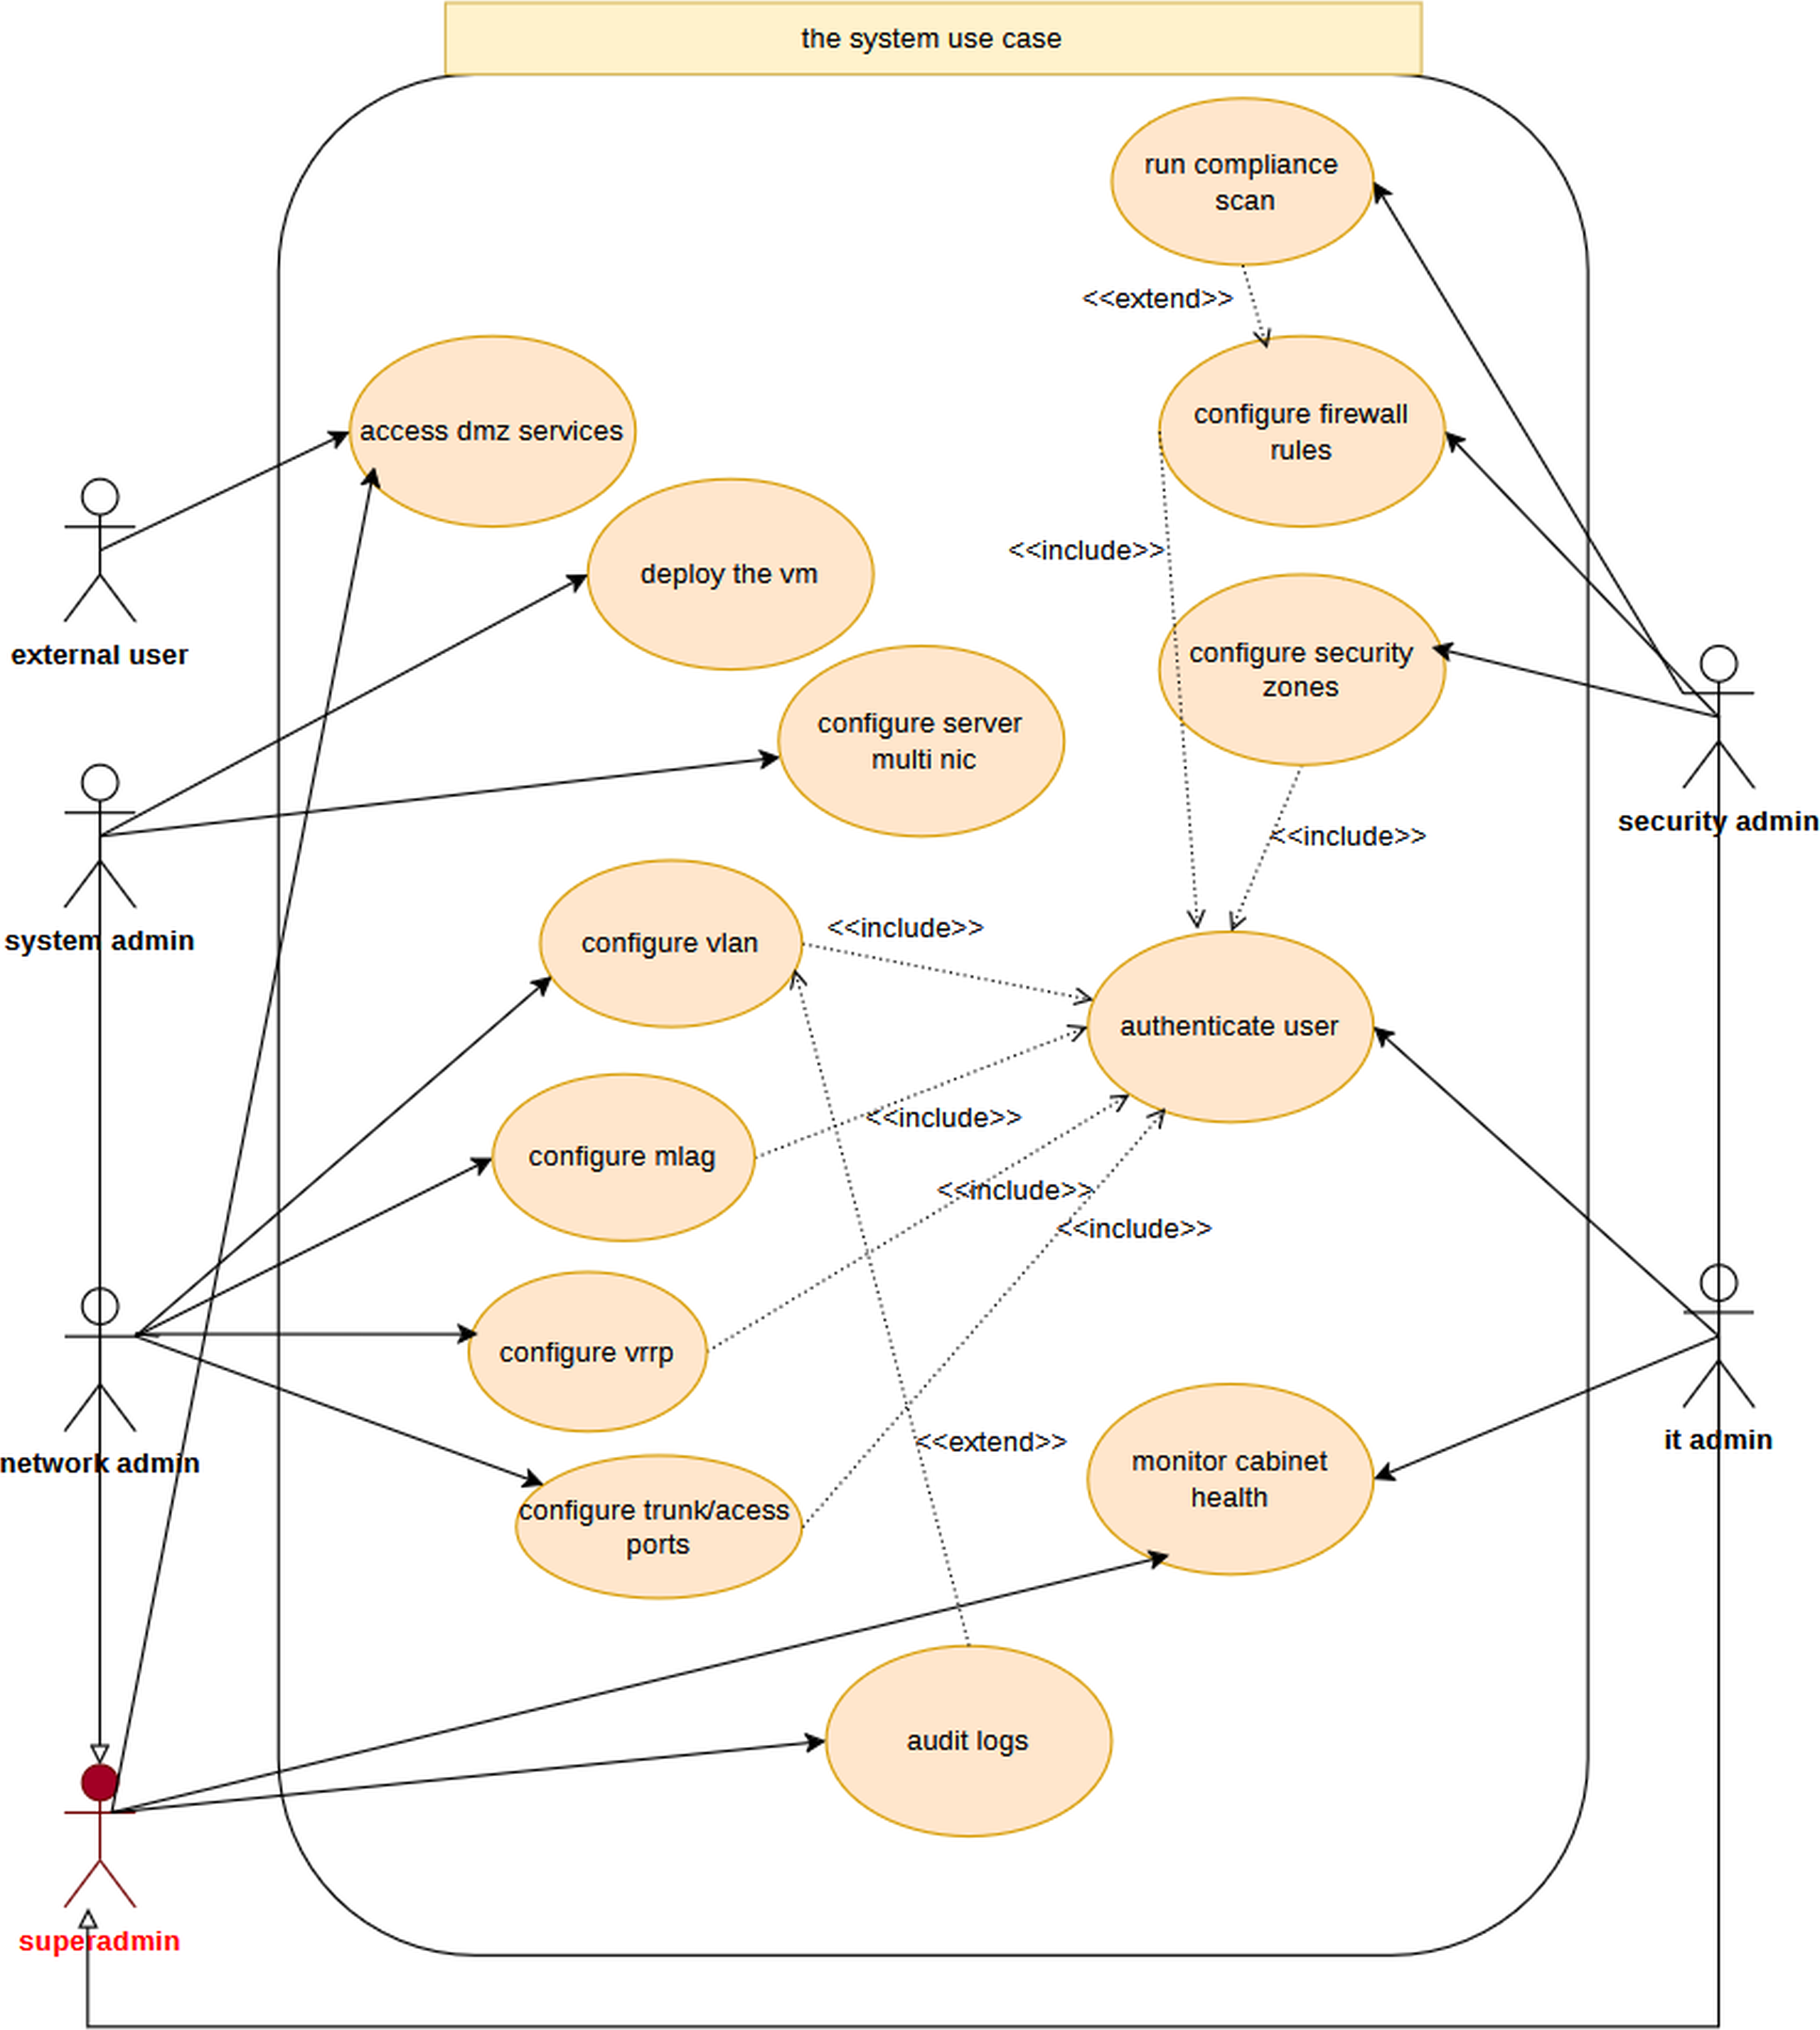
\includegraphics[width=0.72\textwidth,interpolate=false]{figures/newuse.png}
   \caption{Use case diagram of the data center system.}
  \label{fig:usecase}
 \end{figure}
The diagram presents all actors interacting with the data center network architecture. Actors are categorized by their access zone and authentication method.
\section{Sequence Diagrams}
\subsection{Network Administrator Configuring EoR Spine Switches}
The sequence diagram in Figure~\ref{fig:sequence-eor} illustrates the steps a network administrator follows to configure the EoR spine switches (EoR-1 and EoR-2): initial SSH setup, MLAG peer configuration, and downlink binding to ToR switches per cabinet.\\
 \begin{figure}[H]
     \centering
    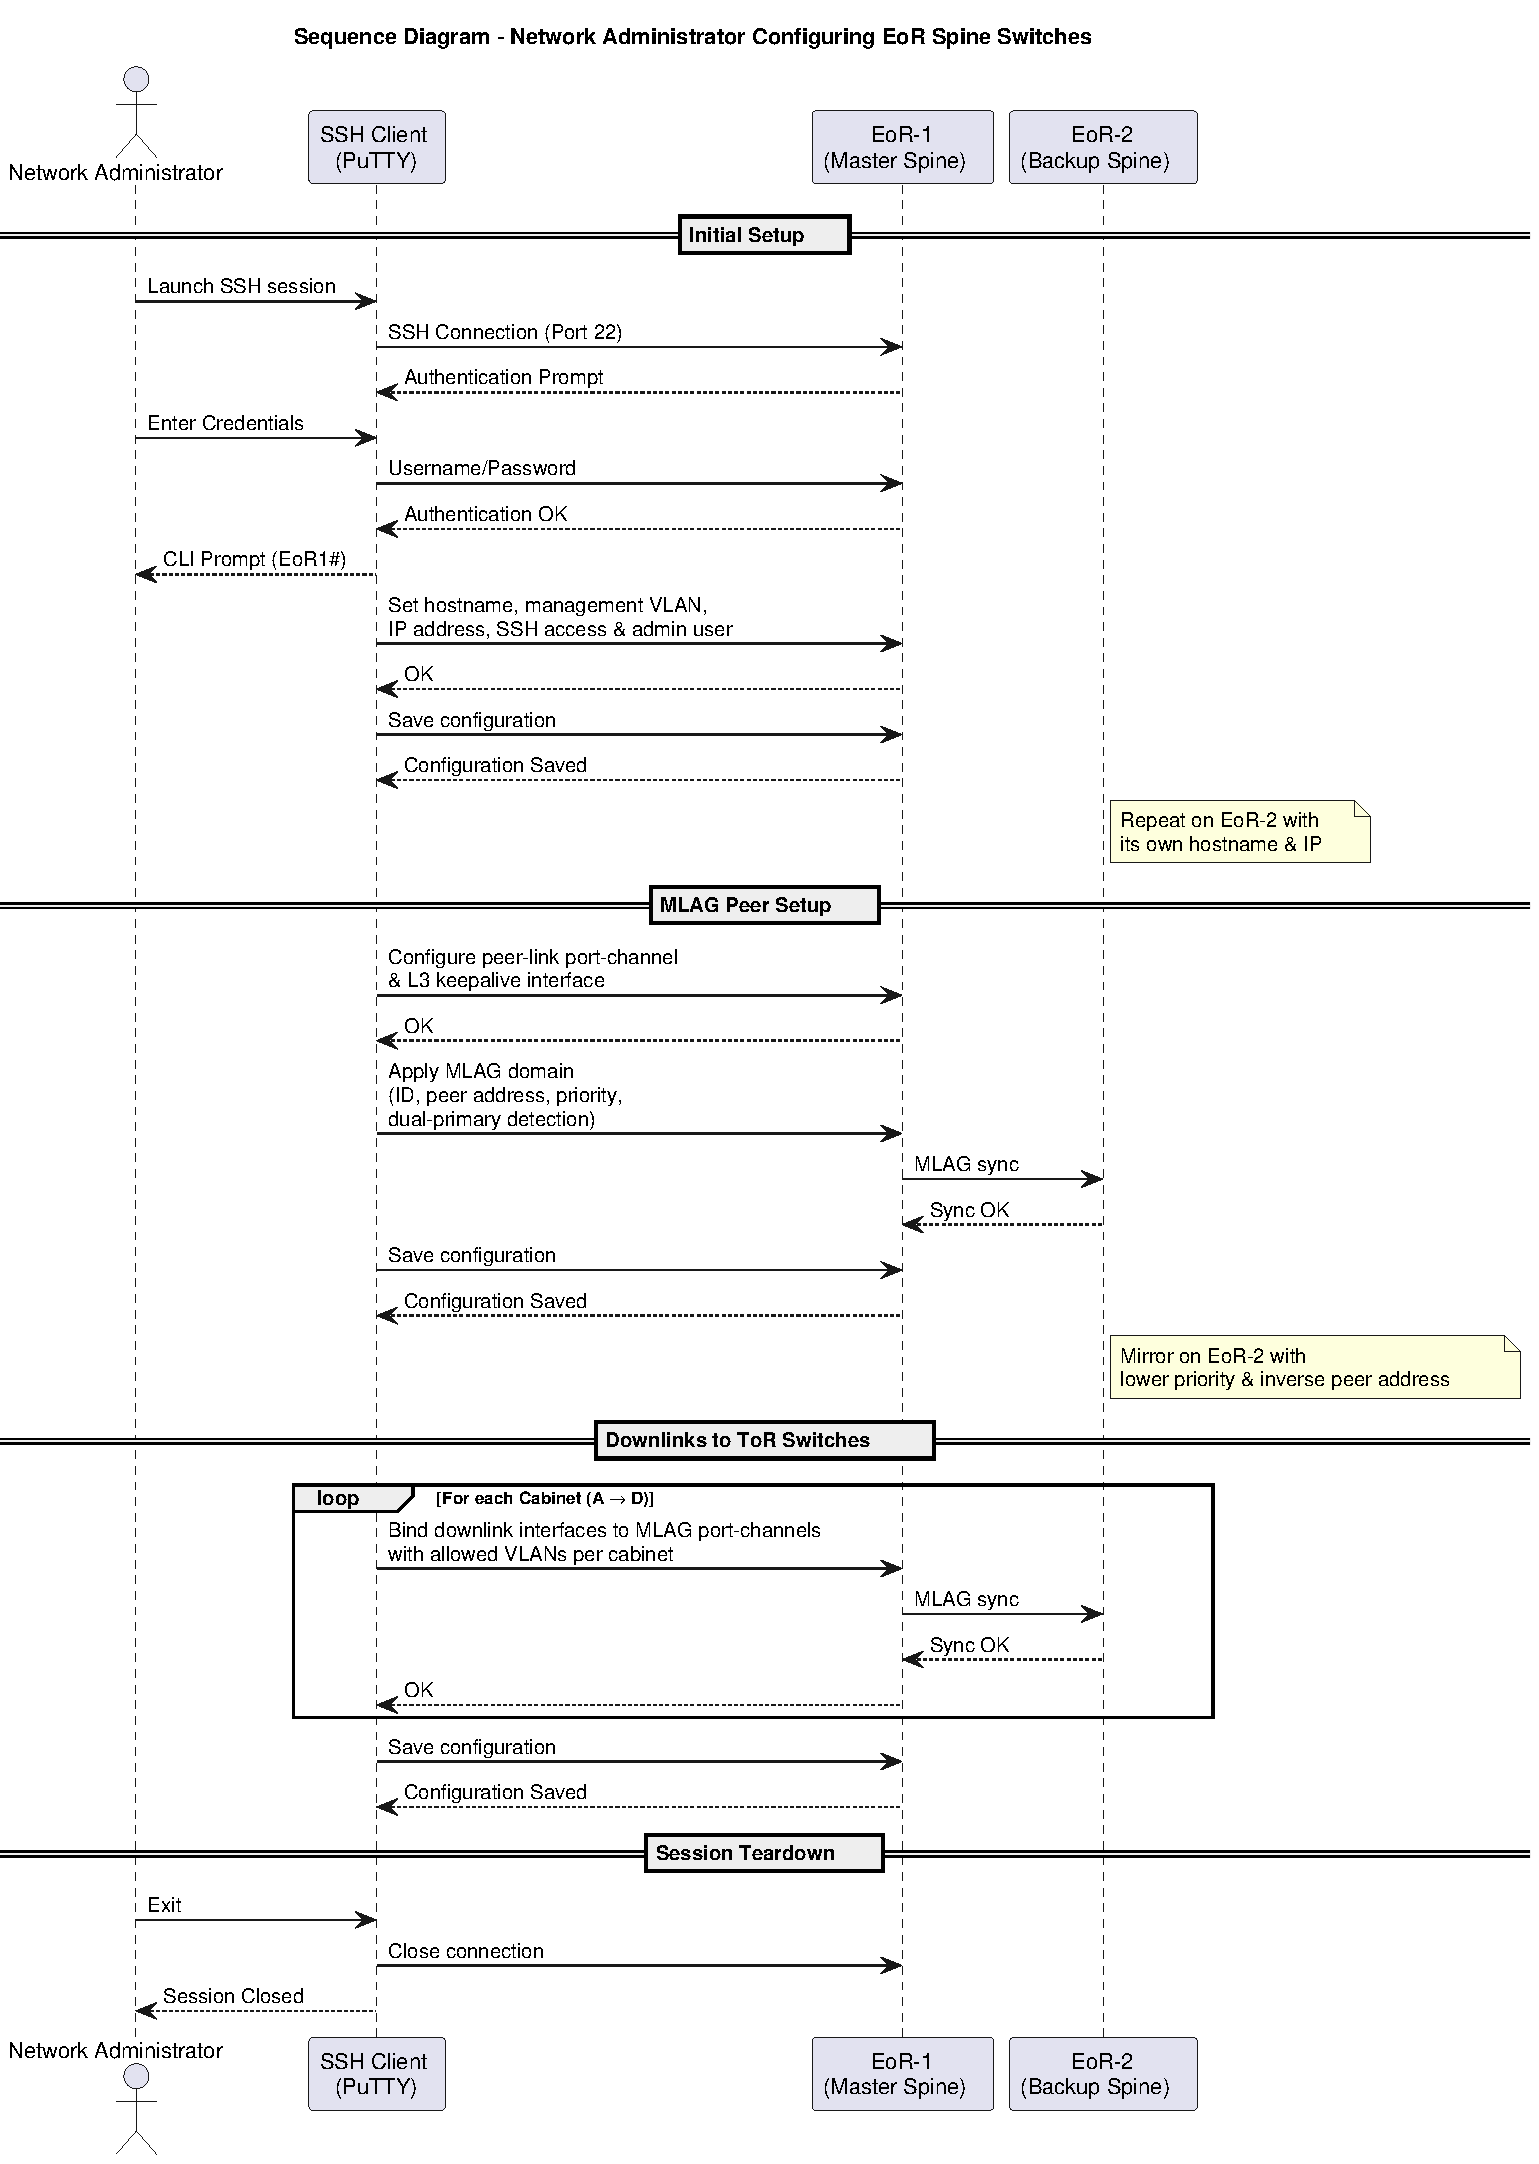
\includegraphics[width=0.88\textwidth,height=0.58\textheight,keepaspectratio]{figures/eor_config_sequence.pdf}
    \caption{Sequence diagram: Network administrator configuring EoR spine switches.}
    \label{fig:sequence-eor}
 \end{figure}

\subsection{System Administrator Configuring a Server}
The sequence diagram in Figure~\ref{fig:sequence-server} illustrates the steps a system administrator follows to configure a Linux server: SSH connection, enabling bonding and 802.1Q kernel modules, configuring physical interfaces, creating \texttt{bond0} (management, VLAN~110) and \texttt{bond1} (service, VLAN~120) with active-backup slaves, and verifying interface reachability before session teardown.\\
 \begin{figure}[H]
     \centering
    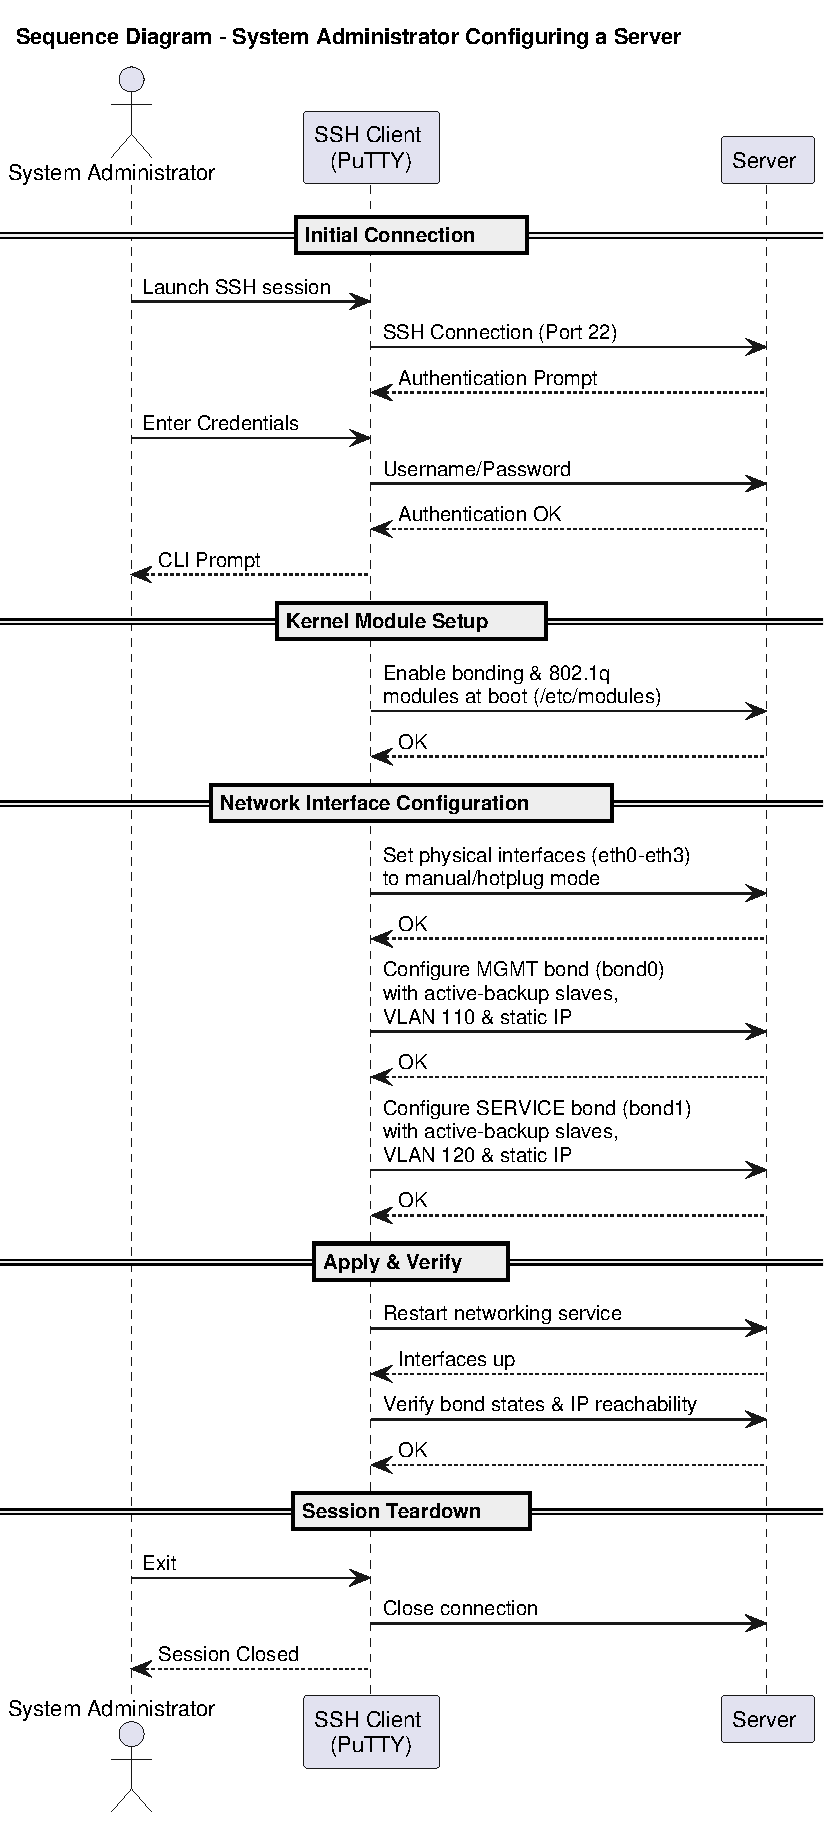
\includegraphics[width=0.88\textwidth,height=0.58\textheight,keepaspectratio]{figures/server_config_sequence.pdf}
    \caption{Sequence diagram: System administrator configuring a server.}
    \label{fig:sequence-server}
 \end{figure}
\section{Low-Level Design (LLD)}

\subsection{Device inventory}
The data center comprises 2 spine switches, 8 leaf switches, 2 firewalls, and 8 servers. Table~\ref{tab:device-inventory-sample} shows one representative device per type; the full inventory is in Appendix~\ref{app:lld}, Figure~\ref{fig:app-device-inventory}.

\begin{table}[htbp]
    \centering
    \small
    \caption{Sample device inventory (one device per type)}
    \label{tab:device-inventory-sample}
    \begin{tabular}{|l|l|l|l|}
        \hline
        \textbf{Device} & \textbf{Model/OS} & \textbf{Role} & \textbf{Location} \\
        \hline
        EoR-1 & Arista vEOS & Spine switch & Core rack \\
        ToR A-1 & Arista vEOS & Leaf switch & Cabinet A \\
        FW-1 & pfSense & Firewall & Core rack \\
        Server 1 & Linux & Database server & Cabinet A \\
        \hline
    \end{tabular}
\end{table}

\subsection{Port connections}
Physical cabling between EoR, ToR, firewall, and server ports is summarized below for one representative path (ToR A-1, EoR-1, FW-1, Server~1). The complete matrices are in Appendix~\ref{app:lld}, Figures~\ref{fig:app-port-conn-1}--\ref{fig:app-port-conn-3}.

\begin{table}[H]
    \centering
    \footnotesize
    \caption{ToR A-1 $\rightarrow$ Server 1 (access, copper trunk).}
    \label{tab:lld-port-tor-server}
    \begin{tabular}{|l|l|l|l|c|}
        \hline
        \textbf{Source port} & \textbf{Type} & \textbf{Destination} & \textbf{Dest.\ port} & \textbf{VLAN} \\
        \hline
        Ethernet0/0/1 & Access & Server 1 & NIC M1 & 110 \\
        Ethernet0/0/2 & Access & Server 1 & NIC S1 & 120 \\
        \hline
    \end{tabular}
\end{table}

\begin{table}[H]
    \centering
    \footnotesize
    \caption{ToR A-1 $\rightarrow$ EoR-1 (uplink, fiber trunk).}
    \label{tab:lld-port-tor-eor}
    \begin{tabular}{|l|l|l|l|c|}
        \hline
        \textbf{Source port} & \textbf{Type} & \textbf{Destination} & \textbf{Dest.\ port} & \textbf{VLANs} \\
        \hline
        GigabitEthernet0/0/1 & Trunk & EoR-1 & GigabitEthernet0/0/1 & 110, 120, 130 \\
        \hline
    \end{tabular}
\end{table}

\begin{table}[H]
    \centering
    \footnotesize
    \caption{EoR-1 $\rightarrow$ FW-1 (edge, fiber trunk).}
    \label{tab:lld-port-eor-fw}
    \begin{tabular}{|l|l|l|l|c|}
        \hline
        \textbf{Source port} & \textbf{Type} & \textbf{Destination} & \textbf{Dest.\ port} & \textbf{VLANs} \\
        \hline
        GigabitEthernet0/0/24 & Trunk & FW-1 & GigabitEthernet1/0/0 & 110, 120, 130, 210, 220 \\
        \hline
    \end{tabular}
\end{table}

Each ToR uplinks to both EoR switches; both EoRs connect to both firewalls; servers dual-home to their cabinet ToR pair.
\hyperref[def:trunk]{\underline{Trunk ports}} carry multiple VLANs between switches. Spine-to-leaf, spine-to-spine, and spine-to-firewall trunks carry all five VLANs (110, 120, 130, 210, 220).

\subsection{VLAN Design}
Based on the security zone requirements and traffic separation needs, we defined the following VLANs from the LLD:
 \begin{figure}[H]
    \centering
   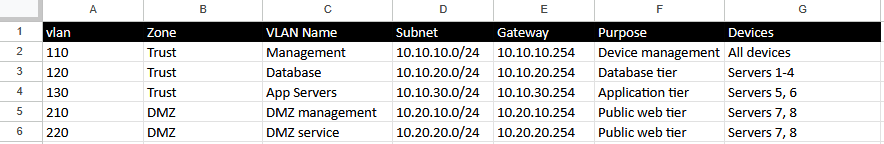
\includegraphics[width=0.72\textwidth,interpolate=false]{figures/vlan.png}
    \caption{VLAN assignment table.}
\label{fig:vlan}
 \end{figure}
All VLANs use /24 subnets (254 usable addresses), providing sufficient capacity for current needs and future expansion.

\subsection{Server IP Assignments}
Each server uses \texttt{bond0} (M1+M2) for management traffic and \texttt{bond1} (S1+S2) for service traffic. ToR and EoR switches use a management SVI on VLAN~110; firewalls use \texttt{lagg0} sub-interfaces per VLAN. Table~\ref{tab:ip-plan-sample} lists one example per device type (IP and interface); the complete plan is in Appendix~\ref{app:lld}, Figure~\ref{fig:app-ip-plan}.

\begin{table}[H]
    \centering
    \scriptsize
    \caption{Sample IP and interface assignments (one device per type).}
    \label{tab:ip-plan-sample}
    \setlength{\tabcolsep}{4pt}
    \renewcommand{\arraystretch}{1.05}
    \resizebox{\textwidth}{!}{%
    \begin{tabular}{|l|cc|cc|cc|cc|cc|}
        \hline
        \textbf{Device} &
        \multicolumn{2}{c|}{\textbf{V110 (mgmt)}} &
        \multicolumn{2}{c|}{\textbf{V120 (DB)}} &
        \multicolumn{2}{c|}{\textbf{V130 (app)}} &
        \multicolumn{2}{c|}{\textbf{V210 (DMZ mgmt)}} &
        \multicolumn{2}{c|}{\textbf{V220 (DMZ web)}} \\
        \cline{2-11}
        & \textbf{IP} & \textbf{Interface} & \textbf{IP} & \textbf{Interface} & \textbf{IP} & \textbf{Interface} & \textbf{IP} & \textbf{Interface} & \textbf{IP} & \textbf{Interface} \\
        \hline
        Server 1 & 10.10.10.1 & bond0 (M1+M2) & 10.10.20.1 & bond1 (S1+S2) & n/a & n/a & n/a & n/a & n/a & n/a \\
        ToR A-1 & 10.10.10.200 & SVI Vlan110 & n/a & n/a & n/a & n/a & n/a & n/a & n/a & n/a \\
        EoR-1 & 10.10.10.208 & SVI Vlan110 & n/a & n/a & n/a & n/a & n/a & n/a & n/a & n/a \\
        FW-1 & 10.10.10.210 & lagg0.110 & 10.10.20.210 & lagg0.120 & 10.10.30.210 & lagg0.130 & 10.20.10.210 & lagg0.210 & 10.20.20.210 & lagg0.220 \\
        \hline
    \end{tabular}%
    }
\end{table}

\section{Gateway \& VRRP Design}
Each VLAN uses a Virtual Router Redundancy Protocol (VRRP) virtual IP address as its default gateway. The firewalls participate in VRRP to provide gateway redundancy and seamless failover, eliminating the need for server reconfiguration during a firewall failure or switchover.

\begin{figure}[H]
    \centering
  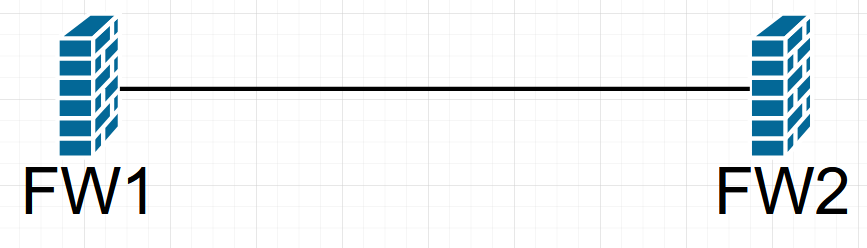
\includegraphics[width=0.6\textwidth,interpolate=false]{figures/firewall_vrrp.png}
     \caption{Firewalls VRRP}
   \label{fig:firewalls-vrrp}
 \end{figure}

\section{MLAG Design}
All switch pairs (ToRs and EoRs) are configured with MLAG setup.\\
- \textbf{Active-standby operation:} One switch forwards traffic while the standby remains ready; on failure, the standby takes over.\\
- \textbf{Sub-second \hyperref[def:failover]{\underline{failover:}}} If the active switch fails, traffic continues through the standby with minimal interruption.

% IMAGE: media/image11.png - MLAG diagram
 \begin{figure}[H]
    \centering
   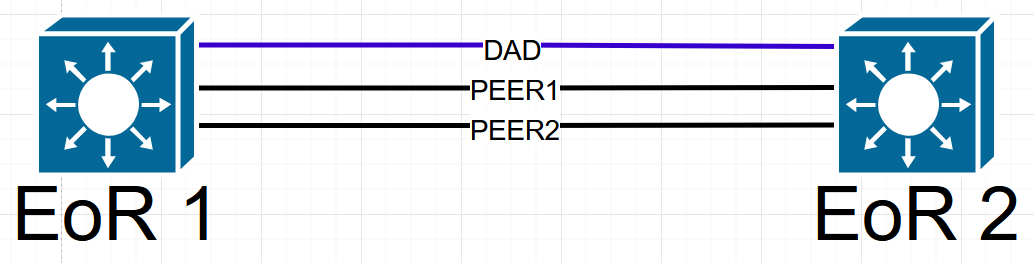
\includegraphics[width=0.6\textwidth,interpolate=false]{figures/eor_mlag.png}
   \caption{EoRs Pair MLAG Architecture}
   \label{fig:mlag}
\end{figure}

\section{Firewall Rules}
Firewall policies enforce strict zone isolation with default-deny rules. Traffic from Untrust to DMZ is permitted only for HTTP and HTTPS. Traffic from DMZ to Trust is permitted only for application-specific ports. All other cross-zone traffic is denied by default. Trust-zone outbound traffic to the external network is permitted via NAT. Management access to all devices is restricted to SSH only.

\section{Conclusion}
This chapter presented a complete spine-leaf data center design with two spines, eight leaves, full-mesh connectivity, and MLAG active-standby pairs at the ToR and EoR layers. Zone-based security separates DMZ, Trust, and Untrust zones via firewall policies, while VRRP supports 99.99\% availability targets.